\documentclass[1p]{elsarticle_modified}
%\bibliographystyle{elsarticle-num}

%\usepackage[colorlinks]{hyperref}
%\usepackage{abbrmath_seonhwa} %\Abb, \Ascr, \Acal ,\Abf, \Afrak
\usepackage{amsfonts}
\usepackage{amssymb}
\usepackage{amsmath}
\usepackage{amsthm}
\usepackage{scalefnt}
\usepackage{amsbsy}
\usepackage{kotex}
\usepackage{caption}
\usepackage{subfig}
\usepackage{color}
\usepackage{graphicx}
\usepackage{xcolor} %% white, black, red, green, blue, cyan, magenta, yellow
\usepackage{float}
\usepackage{setspace}
\usepackage{hyperref}

\usepackage{tikz}
\usetikzlibrary{arrows}

\usepackage{multirow}
\usepackage{array} % fixed length table
\usepackage{hhline}

%%%%%%%%%%%%%%%%%%%%%
\makeatletter
\renewcommand*\env@matrix[1][\arraystretch]{%
	\edef\arraystretch{#1}%
	\hskip -\arraycolsep
	\let\@ifnextchar\new@ifnextchar
	\array{*\c@MaxMatrixCols c}}
\makeatother %https://tex.stackexchange.com/questions/14071/how-can-i-increase-the-line-spacing-in-a-matrix
%%%%%%%%%%%%%%%

\usepackage[normalem]{ulem}

\newcommand{\msout}[1]{\ifmmode\text{\sout{\ensuremath{#1}}}\else\sout{#1}\fi}
%SOURCE: \msout is \stkout macro in https://tex.stackexchange.com/questions/20609/strikeout-in-math-mode

\newcommand{\cancel}[1]{
	\ifmmode
	{\color{red}\msout{#1}}
	\else
	{\color{red}\sout{#1}}
	\fi
}

\newcommand{\add}[1]{
	{\color{blue}\uwave{#1}}
}

\newcommand{\replace}[2]{
	\ifmmode
	{\color{red}\msout{#1}}{\color{blue}\uwave{#2}}
	\else
	{\color{red}\sout{#1}}{\color{blue}\uwave{#2}}
	\fi
}

\newcommand{\Sol}{\mathcal{S}} %segment
\newcommand{\D}{D} %diagram
\newcommand{\A}{\mathcal{A}} %arc


%%%%%%%%%%%%%%%%%%%%%%%%%%%%%5 test

\def\sl{\operatorname{\textup{SL}}(2,\Cbb)}
\def\psl{\operatorname{\textup{PSL}}(2,\Cbb)}
\def\quan{\mkern 1mu \triangleright \mkern 1mu}

\theoremstyle{definition}
\newtheorem{thm}{Theorem}[section]
\newtheorem{prop}[thm]{Proposition}
\newtheorem{lem}[thm]{Lemma}
\newtheorem{ques}[thm]{Question}
\newtheorem{cor}[thm]{Corollary}
\newtheorem{defn}[thm]{Definition}
\newtheorem{exam}[thm]{Example}
\newtheorem{rmk}[thm]{Remark}
\newtheorem{alg}[thm]{Algorithm}

\newcommand{\I}{\sqrt{-1}}
\begin{document}

%\begin{frontmatter}
%
%\title{Boundary parabolic representations of knots up to 8 crossings}
%
%%% Group authors per affiliation:
%\author{Yunhi Cho} 
%\address{Department of Mathematics, University of Seoul, Seoul, Korea}
%\ead{yhcho@uos.ac.kr}
%
%
%\author{Seonhwa Kim} %\fnref{s_kim}}
%\address{Center for Geometry and Physics, Institute for Basic Science, Pohang, 37673, Korea}
%\ead{ryeona17@ibs.re.kr}
%
%\author{Hyuk Kim}
%\address{Department of Mathematical Sciences, Seoul National University, Seoul 08826, Korea}
%\ead{hyukkim@snu.ac.kr}
%
%\author{Seokbeom Yoon}
%\address{Department of Mathematical Sciences, Seoul National University, Seoul, 08826,  Korea}
%\ead{sbyoon15@snu.ac.kr}
%
%\begin{abstract}
%We find all boundary parabolic representation of knots up to 8 crossings.
%
%\end{abstract}
%\begin{keyword}
%    \MSC[2010] 57M25 
%\end{keyword}
%
%\end{frontmatter}

%\linenumbers
%\tableofcontents
%
\newcommand\colored[1]{\textcolor{white}{\rule[-0.35ex]{0.8em}{1.4ex}}\kern-0.8em\color{red} #1}%
%\newcommand\colored[1]{\textcolor{white}{ #1}\kern-2.17ex	\textcolor{white}{ #1}\kern-1.81ex	\textcolor{white}{ #1}\kern-2.15ex\color{red}#1	}

{\Large $\underline{12a_{0392}~(K12a_{0392})}$}

\setlength{\tabcolsep}{10pt}
\renewcommand{\arraystretch}{1.6}
\vspace{1cm}\begin{tabular}{m{100pt}>{\centering\arraybackslash}m{274pt}}
\multirow{5}{120pt}{
	\centering
	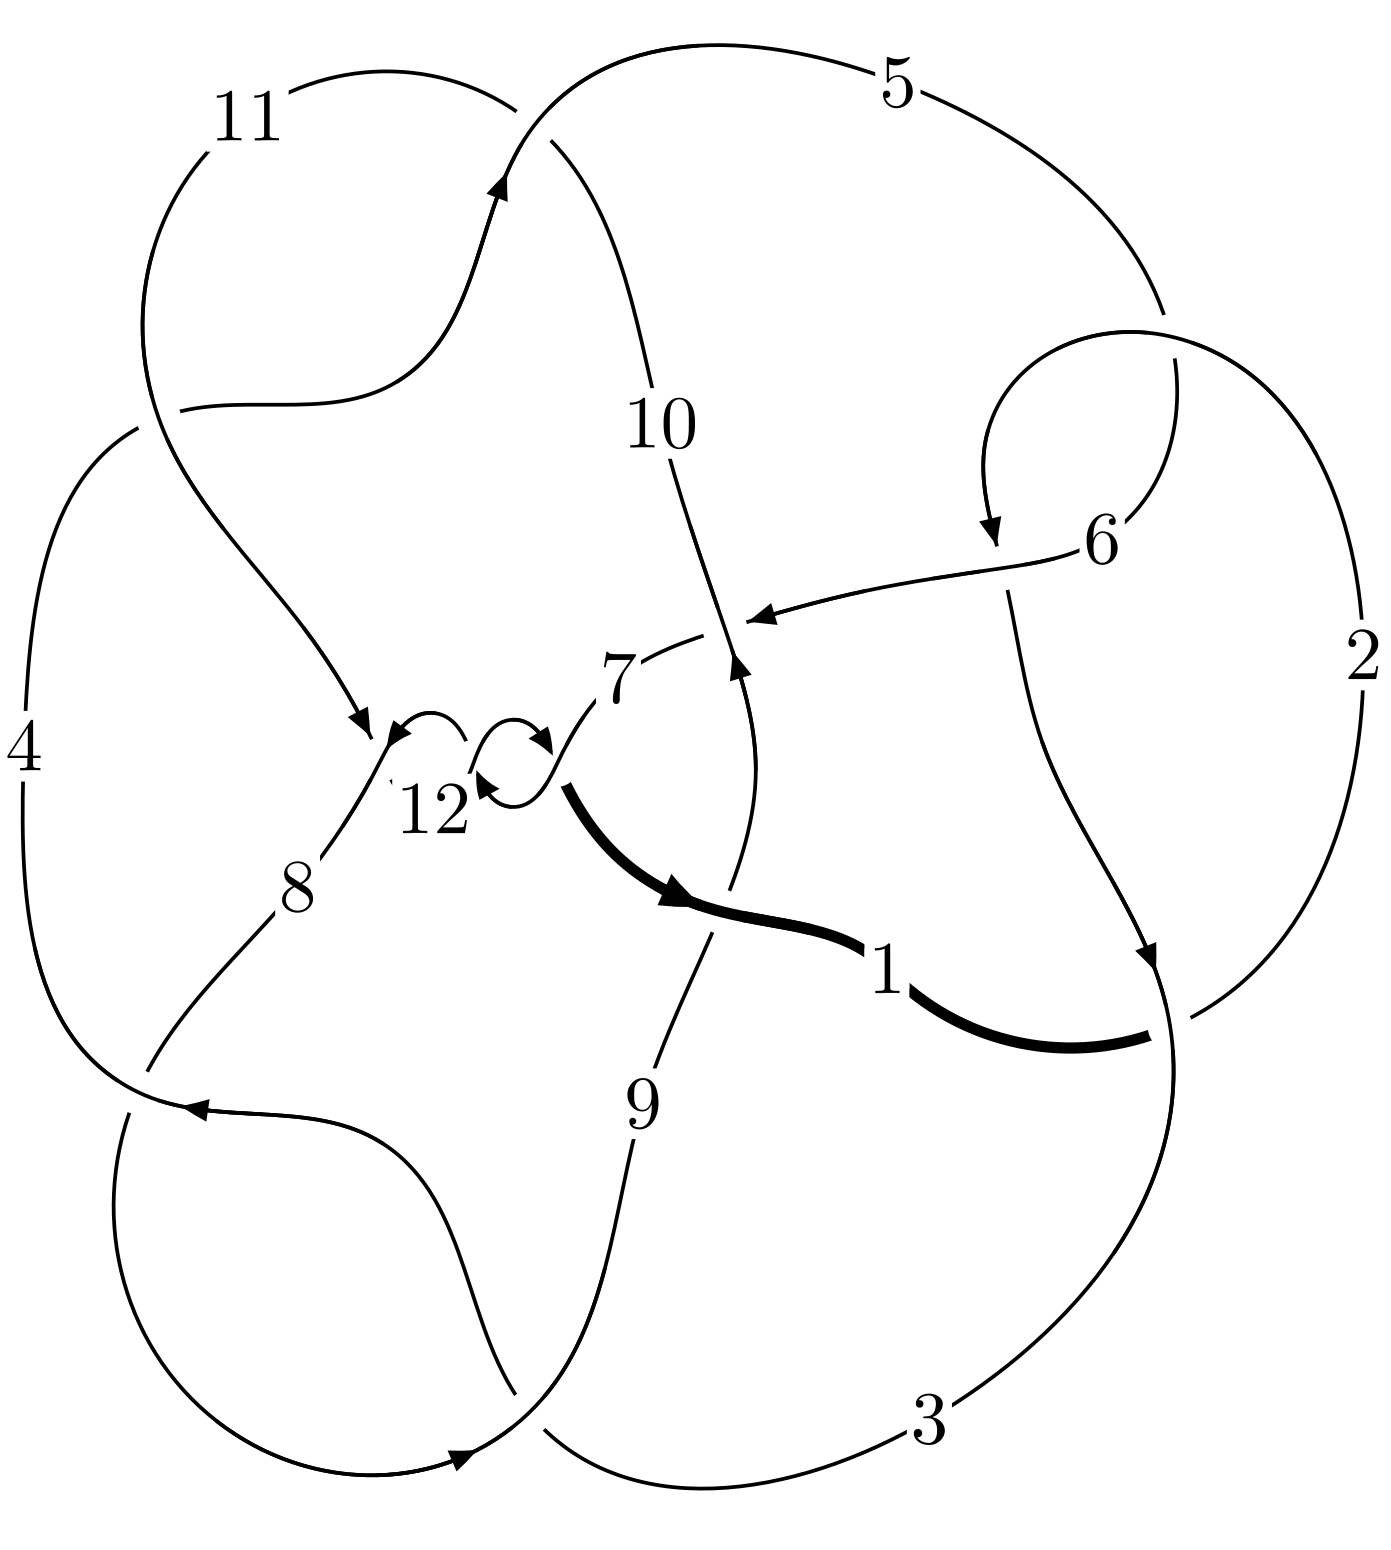
\includegraphics[width=112pt]{../../../GIT/diagram.site/Diagrams/png/1193_12a_0392.png}\\
\ \ \ A knot diagram\footnotemark}&
\allowdisplaybreaks
\textbf{Linearized knot diagam} \\
\cline{2-2}
 &
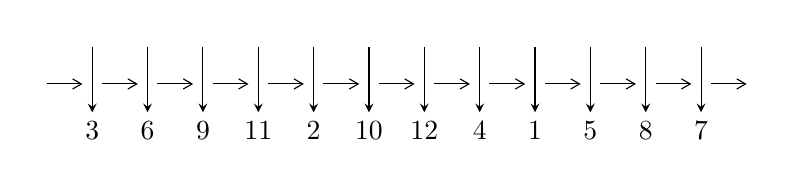
\begin{tikzpicture}[x=20pt, y=17pt]
	% nodes
	\node (C0) at (0, 0) {};
	\node (C1) at (1, 0) {};
	\node (C1U) at (1, +1) {};
	\node (C1D) at (1, -1) {3};

	\node (C2) at (2, 0) {};
	\node (C2U) at (2, +1) {};
	\node (C2D) at (2, -1) {6};

	\node (C3) at (3, 0) {};
	\node (C3U) at (3, +1) {};
	\node (C3D) at (3, -1) {9};

	\node (C4) at (4, 0) {};
	\node (C4U) at (4, +1) {};
	\node (C4D) at (4, -1) {11};

	\node (C5) at (5, 0) {};
	\node (C5U) at (5, +1) {};
	\node (C5D) at (5, -1) {2};

	\node (C6) at (6, 0) {};
	\node (C6U) at (6, +1) {};
	\node (C6D) at (6, -1) {10};

	\node (C7) at (7, 0) {};
	\node (C7U) at (7, +1) {};
	\node (C7D) at (7, -1) {12};

	\node (C8) at (8, 0) {};
	\node (C8U) at (8, +1) {};
	\node (C8D) at (8, -1) {4};

	\node (C9) at (9, 0) {};
	\node (C9U) at (9, +1) {};
	\node (C9D) at (9, -1) {1};

	\node (C10) at (10, 0) {};
	\node (C10U) at (10, +1) {};
	\node (C10D) at (10, -1) {5};

	\node (C11) at (11, 0) {};
	\node (C11U) at (11, +1) {};
	\node (C11D) at (11, -1) {8};

	\node (C12) at (12, 0) {};
	\node (C12U) at (12, +1) {};
	\node (C12D) at (12, -1) {7};
	\node (C13) at (13, 0) {};

	% arrows
	\draw[->,>={angle 60}]
	(C0) edge (C1) (C1) edge (C2) (C2) edge (C3) (C3) edge (C4) (C4) edge (C5) (C5) edge (C6) (C6) edge (C7) (C7) edge (C8) (C8) edge (C9) (C9) edge (C10) (C10) edge (C11) (C11) edge (C12) (C12) edge (C13) ;	\draw[->,>=stealth]
	(C1U) edge (C1D) (C2U) edge (C2D) (C3U) edge (C3D) (C4U) edge (C4D) (C5U) edge (C5D) (C6U) edge (C6D) (C7U) edge (C7D) (C8U) edge (C8D) (C9U) edge (C9D) (C10U) edge (C10D) (C11U) edge (C11D) (C12U) edge (C12D) ;
	\end{tikzpicture} \\
\hhline{~~} \\& 
\textbf{Solving Sequence} \\ \cline{2-2} 
 &
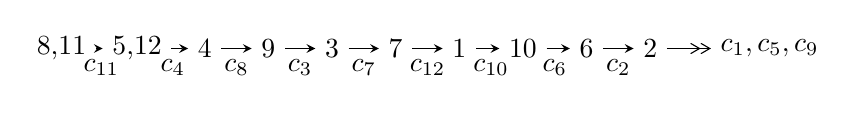
\begin{tikzpicture}[x=23pt, y=7pt]
	% node
	\node (A0) at (-1/8, 0) {8,11};
	\node (A1) at (17/16, 0) {5,12};
	\node (A2) at (17/8, 0) {4};
	\node (A3) at (25/8, 0) {9};
	\node (A4) at (33/8, 0) {3};
	\node (A5) at (41/8, 0) {7};
	\node (A6) at (49/8, 0) {1};
	\node (A7) at (57/8, 0) {10};
	\node (A8) at (65/8, 0) {6};
	\node (A9) at (73/8, 0) {2};
	\node (C1) at (1/2, -1) {$c_{11}$};
	\node (C2) at (13/8, -1) {$c_{4}$};
	\node (C3) at (21/8, -1) {$c_{8}$};
	\node (C4) at (29/8, -1) {$c_{3}$};
	\node (C5) at (37/8, -1) {$c_{7}$};
	\node (C6) at (45/8, -1) {$c_{12}$};
	\node (C7) at (53/8, -1) {$c_{10}$};
	\node (C8) at (61/8, -1) {$c_{6}$};
	\node (C9) at (69/8, -1) {$c_{2}$};
	\node (A10) at (11, 0) {$c_{1},c_{5},c_{9}$};

	% edge
	\draw[->,>=stealth]	
	(A0) edge (A1) (A1) edge (A2) (A2) edge (A3) (A3) edge (A4) (A4) edge (A5) (A5) edge (A6) (A6) edge (A7) (A7) edge (A8) (A8) edge (A9) ;
	\draw[->>,>={angle 60}]	
	(A9) edge (A10);
\end{tikzpicture} \\ 

\end{tabular} \\

\footnotetext{
The image of knot diagram is generated by the software ``\textbf{Draw programme}" developed by Andrew Bartholomew(\url{http://www.layer8.co.uk/maths/draw/index.htm\#Running-draw}), where we modified some parts for our purpose(\url{https://github.com/CATsTAILs/LinksPainter}).
}\phantom \\ \newline 
\centering \textbf{Ideals for irreducible components\footnotemark of $X_{\text{par}}$} 
 
\begin{align*}
I^u_{1}&=\langle 
43 u^{38}+714 u^{37}+\cdots+128 b-4224,\;-119 u^{38}-2108 u^{37}+\cdots+256 a-156160,\\
\phantom{I^u_{1}}&\phantom{= \langle  }u^{39}+18 u^{38}+\cdots+5120 u+256\rangle \\
I^u_{2}&=\langle 
-1.58971\times10^{86} a^{15} u^{3}+2.22794\times10^{86} a^{14} u^{3}+\cdots-5.54346\times10^{88} a-7.99467\times10^{88},\\
\phantom{I^u_{2}}&\phantom{= \langle  }-2 a^{15} u^3+5 a^{14} u^3+\cdots+348 a-417,\;u^4- u^3+3 u^2-2 u+1\rangle \\
I^u_{3}&=\langle 
u^{26}+u^{25}+\cdots+b+2,\;-3 u^{26}+2 u^{25}+\cdots+a-2,\;u^{27}- u^{26}+\cdots-2 u+1\rangle \\
\\
\end{align*}
\raggedright * 3 irreducible components of $\dim_{\mathbb{C}}=0$, with total 130 representations.\\
\footnotetext{All coefficients of polynomials are rational numbers. But the coefficients are sometimes approximated in decimal forms when there is not enough margin.}
\newpage
\renewcommand{\arraystretch}{1}
\centering \section*{I. $I^u_{1}= \langle 43 u^{38}+714 u^{37}+\cdots+128 b-4224,\;-119 u^{38}-2108 u^{37}+\cdots+256 a-156160,\;u^{39}+18 u^{38}+\cdots+5120 u+256 \rangle$}
\flushleft \textbf{(i) Arc colorings}\\
\begin{tabular}{m{7pt} m{180pt} m{7pt} m{180pt} }
\flushright $a_{8}=$&$\begin{pmatrix}0\\u\end{pmatrix}$ \\
\flushright $a_{11}=$&$\begin{pmatrix}1\\0\end{pmatrix}$ \\
\flushright $a_{5}=$&$\begin{pmatrix}\frac{119}{256} u^{38}+\frac{527}{64} u^{37}+\cdots+\frac{20949}{2} u+610\\-\frac{43}{128} u^{38}-\frac{357}{64} u^{37}+\cdots+17 u+33\end{pmatrix}$ \\
\flushright $a_{12}=$&$\begin{pmatrix}1\\u^2\end{pmatrix}$ \\
\flushright $a_{4}=$&$\begin{pmatrix}\frac{33}{256} u^{38}+\frac{85}{32} u^{37}+\cdots+\frac{20983}{2} u+643\\-\frac{43}{128} u^{38}-\frac{357}{64} u^{37}+\cdots+17 u+33\end{pmatrix}$ \\
\flushright $a_{9}=$&$\begin{pmatrix}\frac{3}{2} u^{38}+\frac{51}{2} u^{37}+\cdots+4544 u+\frac{449}{2}\\\frac{3}{2} u^{38}+26 u^{37}+\cdots+\frac{14913}{2} u+384\end{pmatrix}$ \\
\flushright $a_{3}=$&$\begin{pmatrix}-3.08594 u^{38}-51.7266 u^{37}+\cdots+4079 u+359.500\\-\frac{429}{128} u^{38}-\frac{937}{16} u^{37}+\cdots-\frac{28813}{2} u-704\end{pmatrix}$ \\
\flushright $a_{7}=$&$\begin{pmatrix}u\\u^3+u\end{pmatrix}$ \\
\flushright $a_{1}=$&$\begin{pmatrix}u^2+1\\u^4+2 u^2\end{pmatrix}$ \\
\flushright $a_{10}=$&$\begin{pmatrix}0.500000 u^{37}+8.25000 u^{36}+\cdots+2911.50 u+160.500\\-\frac{3}{2} u^{38}-26 u^{37}+\cdots-\frac{14911}{2} u-384\end{pmatrix}$ \\
\flushright $a_{6}=$&$\begin{pmatrix}\frac{1}{2} u^{38}+8 u^{37}+\cdots-\frac{5947}{4} u-96\\\frac{5}{4} u^{38}+\frac{85}{4} u^{37}+\cdots+7201 u+384\end{pmatrix}$ \\
\flushright $a_{2}=$&$\begin{pmatrix}-6 u^{38}-\frac{1669}{16} u^{37}+\cdots-35327 u-\frac{3677}{2}\\-\frac{55}{16} u^{38}-\frac{485}{8} u^{37}+\cdots-\frac{48673}{2} u-1280\end{pmatrix}$\\&\end{tabular}
\flushleft \textbf{(ii) Obstruction class $= -1$}\\~\\
\flushleft \textbf{(iii) Cusp Shapes $= -\frac{49}{8} u^{38}-\frac{1605}{16} u^{37}+\cdots+16358 u+1094$}\\~\\
\newpage\renewcommand{\arraystretch}{1}
\flushleft \textbf{(iv) u-Polynomials at the component}\newline \\
\begin{tabular}{m{50pt}|m{274pt}}
Crossings & \hspace{64pt}u-Polynomials at each crossing \\
\hline $$\begin{aligned}c_{1}\end{aligned}$$&$\begin{aligned}
&u^{39}+18 u^{38}+\cdots+5504 u+256
\end{aligned}$\\
\hline $$\begin{aligned}c_{2},c_{5}\end{aligned}$$&$\begin{aligned}
&u^{39}+12 u^{38}+\cdots+176 u+16
\end{aligned}$\\
\hline $$\begin{aligned}c_{3},c_{4},c_{8}\\c_{10}\end{aligned}$$&$\begin{aligned}
&u^{39}+20 u^{37}+\cdots+4 u+1
\end{aligned}$\\
\hline $$\begin{aligned}c_{6},c_{9}\end{aligned}$$&$\begin{aligned}
&u^{39}- u^{38}+\cdots-8 u+1
\end{aligned}$\\
\hline $$\begin{aligned}c_{7},c_{11},c_{12}\end{aligned}$$&$\begin{aligned}
&u^{39}+18 u^{38}+\cdots+5120 u+256
\end{aligned}$\\
\hline
\end{tabular}\\~\\
\newpage\renewcommand{\arraystretch}{1}
\flushleft \textbf{(v) Riley Polynomials at the component}\newline \\
\begin{tabular}{m{50pt}|m{274pt}}
Crossings & \hspace{64pt}Riley Polynomials at each crossing \\
\hline $$\begin{aligned}c_{1}\end{aligned}$$&$\begin{aligned}
&y^{39}+10 y^{38}+\cdots+19341312 y-65536
\end{aligned}$\\
\hline $$\begin{aligned}c_{2},c_{5}\end{aligned}$$&$\begin{aligned}
&y^{39}-18 y^{38}+\cdots+5504 y-256
\end{aligned}$\\
\hline $$\begin{aligned}c_{3},c_{4},c_{8}\\c_{10}\end{aligned}$$&$\begin{aligned}
&y^{39}+40 y^{38}+\cdots+20 y^2-1
\end{aligned}$\\
\hline $$\begin{aligned}c_{6},c_{9}\end{aligned}$$&$\begin{aligned}
&y^{39}+21 y^{38}+\cdots+4 y-1
\end{aligned}$\\
\hline $$\begin{aligned}c_{7},c_{11},c_{12}\end{aligned}$$&$\begin{aligned}
&y^{39}+36 y^{38}+\cdots+589824 y-65536
\end{aligned}$\\
\hline
\end{tabular}\\~\\
\newpage\flushleft \textbf{(vi) Complex Volumes and Cusp Shapes}
$$\begin{array}{c|c|c}  
\text{Solutions to }I^u_{1}& \I (\text{vol} + \sqrt{-1}CS) & \text{Cusp shape}\\
 \hline 
\begin{aligned}
u &= -0.400663 + 0.963427 I \\
a &= \phantom{-}0.451632 + 0.816397 I \\
b &= \phantom{-}0.369575 - 0.774310 I\end{aligned}
 & -0.15313 + 4.84342 I & \phantom{-0.000000 } 0 \\ \hline\begin{aligned}
u &= -0.400663 - 0.963427 I \\
a &= \phantom{-}0.451632 - 0.816397 I \\
b &= \phantom{-}0.369575 + 0.774310 I\end{aligned}
 & -0.15313 - 4.84342 I & \phantom{-0.000000 } 0 \\ \hline\begin{aligned}
u &= \phantom{-}0.451130 + 0.992863 I \\
a &= \phantom{-}0.138378 + 1.102670 I \\
b &= \phantom{-}0.280699 - 0.629532 I\end{aligned}
 & -1.18720 - 1.89318 I & \phantom{-0.000000 } 0 \\ \hline\begin{aligned}
u &= \phantom{-}0.451130 - 0.992863 I \\
a &= \phantom{-}0.138378 - 1.102670 I \\
b &= \phantom{-}0.280699 + 0.629532 I\end{aligned}
 & -1.18720 + 1.89318 I & \phantom{-0.000000 } 0 \\ \hline\begin{aligned}
u &= -0.052624 + 1.102050 I \\
a &= -0.168827 - 0.844431 I \\
b &= -0.347523 + 0.553746 I\end{aligned}
 & \phantom{-}2.60173 + 1.38324 I & \phantom{-0.000000 } 0 \\ \hline\begin{aligned}
u &= -0.052624 - 1.102050 I \\
a &= -0.168827 + 0.844431 I \\
b &= -0.347523 - 0.553746 I\end{aligned}
 & \phantom{-}2.60173 - 1.38324 I & \phantom{-0.000000 } 0 \\ \hline\begin{aligned}
u &= -0.864676 + 0.737942 I \\
a &= \phantom{-}0.729080 + 0.693284 I \\
b &= \phantom{-}0.35512 - 1.48245 I\end{aligned}
 & \phantom{-}8.1445 + 12.7684 I & \phantom{-0.000000 } 0 \\ \hline\begin{aligned}
u &= -0.864676 - 0.737942 I \\
a &= \phantom{-}0.729080 - 0.693284 I \\
b &= \phantom{-}0.35512 + 1.48245 I\end{aligned}
 & \phantom{-}8.1445 - 12.7684 I & \phantom{-0.000000 } 0 \\ \hline\begin{aligned}
u &= -1.052450 + 0.490837 I \\
a &= \phantom{-}0.533205 + 0.265820 I \\
b &= -0.112515 - 1.397090 I\end{aligned}
 & \phantom{-}7.28855 - 6.50907 I & \phantom{-0.000000 } 0 \\ \hline\begin{aligned}
u &= -1.052450 - 0.490837 I \\
a &= \phantom{-}0.533205 - 0.265820 I \\
b &= -0.112515 + 1.397090 I\end{aligned}
 & \phantom{-}7.28855 + 6.50907 I & \phantom{-0.000000 } 0\\
 \hline 
 \end{array}$$\newpage$$\begin{array}{c|c|c}  
\text{Solutions to }I^u_{1}& \I (\text{vol} + \sqrt{-1}CS) & \text{Cusp shape}\\
 \hline 
\begin{aligned}
u &= -0.910975 + 0.731798 I \\
a &= -0.702822 - 0.636181 I \\
b &= -0.26897 + 1.47836 I\end{aligned}
 & \phantom{-}9.80197 + 6.44149 I & \phantom{-0.000000 } 0 \\ \hline\begin{aligned}
u &= -0.910975 - 0.731798 I \\
a &= -0.702822 + 0.636181 I \\
b &= -0.26897 - 1.47836 I\end{aligned}
 & \phantom{-}9.80197 - 6.44149 I & \phantom{-0.000000 } 0 \\ \hline\begin{aligned}
u &= -1.061090 + 0.576155 I \\
a &= -0.567903 - 0.380804 I \\
b &= \phantom{-}0.01767 + 1.42483 I\end{aligned}
 & \phantom{-}9.20680 + 0.05896 I & \phantom{-0.000000 } 0 \\ \hline\begin{aligned}
u &= -1.061090 - 0.576155 I \\
a &= -0.567903 + 0.380804 I \\
b &= \phantom{-}0.01767 - 1.42483 I\end{aligned}
 & \phantom{-}9.20680 - 0.05896 I & \phantom{-0.000000 } 0 \\ \hline\begin{aligned}
u &= -0.690930 + 0.149615 I \\
a &= \phantom{-}0.021817 - 0.306127 I \\
b &= -0.353074 - 0.523995 I\end{aligned}
 & -2.57796 - 0.99729 I & -13.7858 + 6.1595 I \\ \hline\begin{aligned}
u &= -0.690930 - 0.149615 I \\
a &= \phantom{-}0.021817 + 0.306127 I \\
b &= -0.353074 + 0.523995 I\end{aligned}
 & -2.57796 + 0.99729 I & -13.7858 - 6.1595 I \\ \hline\begin{aligned}
u &= -0.255978 + 1.318020 I \\
a &= -0.463212 - 0.163607 I \\
b &= \phantom{-}0.218629 + 0.376986 I\end{aligned}
 & \phantom{-}1.98110 + 2.40422 I & \phantom{-0.000000 } 0 \\ \hline\begin{aligned}
u &= -0.255978 - 1.318020 I \\
a &= -0.463212 + 0.163607 I \\
b &= \phantom{-}0.218629 - 0.376986 I\end{aligned}
 & \phantom{-}1.98110 - 2.40422 I & \phantom{-0.000000 } 0 \\ \hline\begin{aligned}
u &= -0.537476 + 0.324278 I \\
a &= -0.171379 - 0.673239 I \\
b &= -0.761237 - 0.128475 I\end{aligned}
 & -0.73710 + 3.72784 I & -13.9761 - 6.1233 I \\ \hline\begin{aligned}
u &= -0.537476 - 0.324278 I \\
a &= -0.171379 + 0.673239 I \\
b &= -0.761237 + 0.128475 I\end{aligned}
 & -0.73710 - 3.72784 I & -13.9761 + 6.1233 I\\
 \hline 
 \end{array}$$\newpage$$\begin{array}{c|c|c}  
\text{Solutions to }I^u_{1}& \I (\text{vol} + \sqrt{-1}CS) & \text{Cusp shape}\\
 \hline 
\begin{aligned}
u &= -1.115760 + 0.810029 I \\
a &= \phantom{-}0.508718 + 0.600988 I \\
b &= \phantom{-}0.130410 - 1.320350 I\end{aligned}
 & \phantom{-}1.72502 + 3.78448 I & \phantom{-0.000000 } 0 \\ \hline\begin{aligned}
u &= -1.115760 - 0.810029 I \\
a &= \phantom{-}0.508718 - 0.600988 I \\
b &= \phantom{-}0.130410 + 1.320350 I\end{aligned}
 & \phantom{-}1.72502 - 3.78448 I & \phantom{-0.000000 } 0 \\ \hline\begin{aligned}
u &= -0.149861 + 1.383670 I \\
a &= \phantom{-}0.469652 - 0.674866 I \\
b &= -0.672332 + 0.210913 I\end{aligned}
 & \phantom{-}5.20966 + 1.40328 I & \phantom{-0.000000 } 0 \\ \hline\begin{aligned}
u &= -0.149861 - 1.383670 I \\
a &= \phantom{-}0.469652 + 0.674866 I \\
b &= -0.672332 - 0.210913 I\end{aligned}
 & \phantom{-}5.20966 - 1.40328 I & \phantom{-0.000000 } 0 \\ \hline\begin{aligned}
u &= -0.190013 + 1.391680 I \\
a &= -0.653793 + 0.515105 I \\
b &= \phantom{-}0.726029 - 0.003275 I\end{aligned}
 & \phantom{-}4.70756 + 6.35711 I & \phantom{-0.000000 } 0 \\ \hline\begin{aligned}
u &= -0.190013 - 1.391680 I \\
a &= -0.653793 - 0.515105 I \\
b &= \phantom{-}0.726029 + 0.003275 I\end{aligned}
 & \phantom{-}4.70756 - 6.35711 I & \phantom{-0.000000 } 0 \\ \hline\begin{aligned}
u &= -0.399279 + 0.387480 I \\
a &= \phantom{-}0.394234 + 0.785740 I \\
b &= \phantom{-}0.665015 - 0.160987 I\end{aligned}
 & -0.299504 - 0.631618 I & -12.71997 - 1.63926 I \\ \hline\begin{aligned}
u &= -0.399279 - 0.387480 I \\
a &= \phantom{-}0.394234 - 0.785740 I \\
b &= \phantom{-}0.665015 + 0.160987 I\end{aligned}
 & -0.299504 + 0.631618 I & -12.71997 + 1.63926 I \\ \hline\begin{aligned}
u &= -0.27536 + 1.63405 I \\
a &= -0.50107 - 1.80207 I \\
b &= -0.53416 + 1.64963 I\end{aligned}
 & \phantom{-}15.9909 + 17.0430 I & \phantom{-0.000000 } 0 \\ \hline\begin{aligned}
u &= -0.27536 - 1.63405 I \\
a &= -0.50107 + 1.80207 I \\
b &= -0.53416 - 1.64963 I\end{aligned}
 & \phantom{-}15.9909 - 17.0430 I & \phantom{-0.000000 } 0\\
 \hline 
 \end{array}$$\newpage$$\begin{array}{c|c|c}  
\text{Solutions to }I^u_{1}& \I (\text{vol} + \sqrt{-1}CS) & \text{Cusp shape}\\
 \hline 
\begin{aligned}
u &= -0.28713 + 1.63936 I \\
a &= \phantom{-}0.54343 + 1.73997 I \\
b &= \phantom{-}0.47039 - 1.63060 I\end{aligned}
 & \phantom{-}17.6388 + 10.9152 I & \phantom{-0.000000 } 0 \\ \hline\begin{aligned}
u &= -0.28713 - 1.63936 I \\
a &= \phantom{-}0.54343 - 1.73997 I \\
b &= \phantom{-}0.47039 + 1.63060 I\end{aligned}
 & \phantom{-}17.6388 - 10.9152 I & \phantom{-0.000000 } 0 \\ \hline\begin{aligned}
u &= -0.308532\phantom{ +0.000000I} \\
a &= \phantom{-}0.796218\phantom{ +0.000000I} \\
b &= \phantom{-}0.355272\phantom{ +0.000000I}\end{aligned}
 & -0.538927\phantom{ +0.000000I} & -18.2760\phantom{ +0.000000I} \\ \hline\begin{aligned}
u &= -0.35579 + 1.66576 I \\
a &= \phantom{-}0.62206 + 1.45371 I \\
b &= \phantom{-}0.26274 - 1.48497 I\end{aligned}
 & \phantom{-}16.6078 + 5.4335 I & \phantom{-0.000000 } 0 \\ \hline\begin{aligned}
u &= -0.35579 - 1.66576 I \\
a &= \phantom{-}0.62206 - 1.45371 I \\
b &= \phantom{-}0.26274 + 1.48497 I\end{aligned}
 & \phantom{-}16.6078 - 5.4335 I & \phantom{-0.000000 } 0 \\ \hline\begin{aligned}
u &= -0.41026 + 1.66303 I \\
a &= -0.64890 - 1.31609 I \\
b &= -0.17699 + 1.41341 I\end{aligned}
 & \phantom{-}14.2343 - 0.9071 I & \phantom{-0.000000 } 0 \\ \hline\begin{aligned}
u &= -0.41026 - 1.66303 I \\
a &= -0.64890 + 1.31609 I \\
b &= -0.17699 - 1.41341 I\end{aligned}
 & \phantom{-}14.2343 + 0.9071 I & \phantom{-0.000000 } 0 \\ \hline\begin{aligned}
u &= -0.28654 + 1.68929 I \\
a &= -0.43241 - 1.56815 I \\
b &= -0.44711 + 1.45266 I\end{aligned}
 & \phantom{-}10.16570 + 8.90260 I & \phantom{-0.000000 } 0 \\ \hline\begin{aligned}
u &= -0.28654 - 1.68929 I \\
a &= -0.43241 + 1.56815 I \\
b &= -0.44711 - 1.45266 I\end{aligned}
 & \phantom{-}10.16570 - 8.90260 I & \phantom{-0.000000 } 0\\
 \hline 
 \end{array}$$\newpage\newpage\renewcommand{\arraystretch}{1}
\centering \section*{II. $I^u_{2}= \langle -1.59\times10^{86} a^{15} u^{3}+2.23\times10^{86} a^{14} u^{3}+\cdots-5.54\times10^{88} a-7.99\times10^{88},\;-2 a^{15} u^3+5 a^{14} u^3+\cdots+348 a-417,\;u^4- u^3+3 u^2-2 u+1 \rangle$}
\flushleft \textbf{(i) Arc colorings}\\
\begin{tabular}{m{7pt} m{180pt} m{7pt} m{180pt} }
\flushright $a_{8}=$&$\begin{pmatrix}0\\u\end{pmatrix}$ \\
\flushright $a_{11}=$&$\begin{pmatrix}1\\0\end{pmatrix}$ \\
\flushright $a_{5}=$&$\begin{pmatrix}a\\0.00408887 a^{15} u^{3}-0.00573044 a^{14} u^{3}+\cdots+1.42582 a+2.05629\end{pmatrix}$ \\
\flushright $a_{12}=$&$\begin{pmatrix}1\\u^2\end{pmatrix}$ \\
\flushright $a_{4}=$&$\begin{pmatrix}0.00408887 a^{15} u^{3}-0.00573044 a^{14} u^{3}+\cdots+2.42582 a+2.05629\\0.00408887 a^{15} u^{3}-0.00573044 a^{14} u^{3}+\cdots+1.42582 a+2.05629\end{pmatrix}$ \\
\flushright $a_{9}=$&$\begin{pmatrix}-0.00155418 a^{15} u^{3}+0.00258699 a^{14} u^{3}+\cdots+0.0885681 a+1.18429\\-0.00126205 a^{15} u^{3}+0.000265938 a^{14} u^{3}+\cdots+1.25572 a+0.310048\end{pmatrix}$ \\
\flushright $a_{3}=$&$\begin{pmatrix}-0.00131987 a^{15} u^{3}+0.00795777 a^{14} u^{3}+\cdots-4.11698 a-0.379473\\0.00514080 a^{15} u^{3}-0.000145096 a^{14} u^{3}+\cdots+1.65513 a+0.682050\end{pmatrix}$ \\
\flushright $a_{7}=$&$\begin{pmatrix}u\\u^3+u\end{pmatrix}$ \\
\flushright $a_{1}=$&$\begin{pmatrix}u^2+1\\u^3- u^2+2 u-1\end{pmatrix}$ \\
\flushright $a_{10}=$&$\begin{pmatrix}-0.000982963 a^{15} u^{3}+0.00140342 a^{14} u^{3}+\cdots-0.640785 a+0.472882\\0.00120849 a^{15} u^{3}+0.00435844 a^{14} u^{3}+\cdots+0.567163 a-0.159396\end{pmatrix}$ \\
\flushright $a_{6}=$&$\begin{pmatrix}0.00145898 a^{15} u^{3}-0.00366768 a^{14} u^{3}+\cdots+0.244446 a+0.563875\\-0.00148404 a^{15} u^{3}+0.00319394 a^{14} u^{3}+\cdots-0.647576 a-0.831641\end{pmatrix}$ \\
\flushright $a_{2}=$&$\begin{pmatrix}0.000836775 a^{15} u^{3}+0.00741350 a^{14} u^{3}+\cdots-2.24164 a-1.04569\\0.00384949 a^{15} u^{3}-0.00353384 a^{14} u^{3}+\cdots+2.01767 a-1.78758\end{pmatrix}$\\&\end{tabular}
\flushleft \textbf{(ii) Obstruction class $= -1$}\\~\\
\flushleft \textbf{(iii) Cusp Shapes $= 0.00740162 a^{15} u^{3}-0.000148538 a^{14} u^{3}+\cdots-0.708796 a-10.4488$}\\~\\
\newpage\renewcommand{\arraystretch}{1}
\flushleft \textbf{(iv) u-Polynomials at the component}\newline \\
\begin{tabular}{m{50pt}|m{274pt}}
Crossings & \hspace{64pt}u-Polynomials at each crossing \\
\hline $$\begin{aligned}c_{1}\end{aligned}$$&$\begin{aligned}
&(u^8+3 u^7+7 u^6+10 u^5+11 u^4+10 u^3+6 u^2+4 u+1)^8
\end{aligned}$\\
\hline $$\begin{aligned}c_{2},c_{5}\end{aligned}$$&$\begin{aligned}
&(u^8- u^7- u^6+2 u^5+u^4-2 u^3+2 u-1)^8
\end{aligned}$\\
\hline $$\begin{aligned}c_{3},c_{4},c_{8}\\c_{10}\end{aligned}$$&$\begin{aligned}
&u^{64}- u^{63}+\cdots-56048 u+9017
\end{aligned}$\\
\hline $$\begin{aligned}c_{6},c_{9}\end{aligned}$$&$\begin{aligned}
&u^{64}+9 u^{63}+\cdots-186580 u+125537
\end{aligned}$\\
\hline $$\begin{aligned}c_{7},c_{11},c_{12}\end{aligned}$$&$\begin{aligned}
&(u^4- u^3+3 u^2-2 u+1)^{16}
\end{aligned}$\\
\hline
\end{tabular}\\~\\
\newpage\renewcommand{\arraystretch}{1}
\flushleft \textbf{(v) Riley Polynomials at the component}\newline \\
\begin{tabular}{m{50pt}|m{274pt}}
Crossings & \hspace{64pt}Riley Polynomials at each crossing \\
\hline $$\begin{aligned}c_{1}\end{aligned}$$&$\begin{aligned}
&(y^8+5 y^7+11 y^6+6 y^5-17 y^4-34 y^3-22 y^2-4 y+1)^8
\end{aligned}$\\
\hline $$\begin{aligned}c_{2},c_{5}\end{aligned}$$&$\begin{aligned}
&(y^8-3 y^7+7 y^6-10 y^5+11 y^4-10 y^3+6 y^2-4 y+1)^8
\end{aligned}$\\
\hline $$\begin{aligned}c_{3},c_{4},c_{8}\\c_{10}\end{aligned}$$&$\begin{aligned}
&y^{64}+63 y^{63}+\cdots+550974992 y+81306289
\end{aligned}$\\
\hline $$\begin{aligned}c_{6},c_{9}\end{aligned}$$&$\begin{aligned}
&y^{64}+23 y^{63}+\cdots+140468688776 y+15759538369
\end{aligned}$\\
\hline $$\begin{aligned}c_{7},c_{11},c_{12}\end{aligned}$$&$\begin{aligned}
&(y^4+5 y^3+7 y^2+2 y+1)^{16}
\end{aligned}$\\
\hline
\end{tabular}\\~\\
\newpage\flushleft \textbf{(vi) Complex Volumes and Cusp Shapes}
$$\begin{array}{c|c|c}  
\text{Solutions to }I^u_{2}& \I (\text{vol} + \sqrt{-1}CS) & \text{Cusp shape}\\
 \hline 
\begin{aligned}
u &= \phantom{-}0.395123 + 0.506844 I \\
a &= \phantom{-}0.529964 - 0.894339 I \\
b &= -0.271440 + 1.194030 I\end{aligned}
 & \phantom{-}3.68314 - 0.28387 I & -7.24196 + 4.39795 I \\ \hline\begin{aligned}
u &= \phantom{-}0.395123 + 0.506844 I \\
a &= -0.834931 - 0.385761 I \\
b &= -0.868179 - 0.429906 I\end{aligned}
 & \phantom{-}3.68314 - 2.54634 I & -7.24196 + 5.41953 I \\ \hline\begin{aligned}
u &= \phantom{-}0.395123 + 0.506844 I \\
a &= -1.106250 + 0.193590 I \\
b &= -0.53504 - 1.55487 I\end{aligned}
 & \phantom{-}6.88321 - 3.99360 I & -4.10382 + 8.47670 I \\ \hline\begin{aligned}
u &= \phantom{-}0.395123 + 0.506844 I \\
a &= \phantom{-}1.090130 - 0.270344 I \\
b &= \phantom{-}0.39737 + 1.63331 I\end{aligned}
 & \phantom{-}6.88321 + 1.16339 I & -4.10382 + 1.34079 I \\ \hline\begin{aligned}
u &= \phantom{-}0.395123 + 0.506844 I \\
a &= \phantom{-}0.497578 + 0.719297 I \\
b &= \phantom{-}0.672533 - 0.182376 I\end{aligned}
 & -1.77893 - 1.41510 I & -13.6908 + 4.9087 I \\ \hline\begin{aligned}
u &= \phantom{-}0.395123 + 0.506844 I \\
a &= -0.325623 + 0.736979 I \\
b &= \phantom{-}0.516120 - 1.133730 I\end{aligned}
 & \phantom{-}2.34412 + 5.02843 I & -9.25519 - 0.38543 I \\ \hline\begin{aligned}
u &= \phantom{-}0.395123 + 0.506844 I \\
a &= \phantom{-}0.692179 + 0.327627 I \\
b &= \phantom{-}1.083680 + 0.298282 I\end{aligned}
 & \phantom{-}2.34412 - 7.85864 I & -9.25519 + 10.20291 I \\ \hline\begin{aligned}
u &= \phantom{-}0.395123 + 0.506844 I \\
a &= -1.51485 - 0.13034 I \\
b &= -0.280648 - 1.037500 I\end{aligned}
 & \phantom{-}3.87876 - 1.41510 I & -11.72120 + 4.90874 I \\ \hline\begin{aligned}
u &= \phantom{-}0.395123 + 0.506844 I \\
a &= \phantom{-}1.42416 - 0.72333 I \\
b &= \phantom{-}0.117535 + 1.371480 I\end{aligned}
 & \phantom{-}3.87876 - 1.41510 I & -11.72120 + 4.90874 I \\ \hline\begin{aligned}
u &= \phantom{-}0.395123 + 0.506844 I \\
a &= -1.25536 - 1.22597 I \\
b &= \phantom{-}0.049747 - 0.249446 I\end{aligned}
 & \phantom{-}3.68314 - 0.28387 I & -7.24196 + 4.39795 I\\
 \hline 
 \end{array}$$\newpage$$\begin{array}{c|c|c}  
\text{Solutions to }I^u_{2}& \I (\text{vol} + \sqrt{-1}CS) & \text{Cusp shape}\\
 \hline 
\begin{aligned}
u &= \phantom{-}0.395123 + 0.506844 I \\
a &= -0.22939 + 1.80501 I \\
b &= -0.190203 - 0.805214 I\end{aligned}
 & -1.77893 - 1.41510 I & -13.6908 + 4.9087 I \\ \hline\begin{aligned}
u &= \phantom{-}0.395123 + 0.506844 I \\
a &= \phantom{-}1.17390 + 1.65779 I \\
b &= -0.276362 + 0.060214 I\end{aligned}
 & \phantom{-}2.34412 + 5.02843 I & -9.25519 - 0.38543 I \\ \hline\begin{aligned}
u &= \phantom{-}0.395123 + 0.506844 I \\
a &= \phantom{-}1.09863 - 1.83963 I \\
b &= \phantom{-}0.259522 + 1.185500 I\end{aligned}
 & \phantom{-}3.68314 - 2.54634 I & -7.24196 + 5.41953 I \\ \hline\begin{aligned}
u &= \phantom{-}0.395123 + 0.506844 I \\
a &= -1.01834 + 2.19191 I \\
b &= -0.384446 - 1.147400 I\end{aligned}
 & \phantom{-}2.34412 - 7.85864 I & -9.25519 + 10.20291 I \\ \hline\begin{aligned}
u &= \phantom{-}0.395123 + 0.506844 I \\
a &= -2.48760 + 0.21755 I \\
b &= \phantom{-}0.103066 - 1.292470 I\end{aligned}
 & \phantom{-}6.88321 + 1.16339 I & -4.10382 + 1.34079 I \\ \hline\begin{aligned}
u &= \phantom{-}0.395123 + 0.506844 I \\
a &= \phantom{-}2.46143 - 0.53883 I \\
b &= -0.041443 + 1.369750 I\end{aligned}
 & \phantom{-}6.88321 - 3.99360 I & -4.10382 + 8.47670 I \\ \hline\begin{aligned}
u &= \phantom{-}0.395123 - 0.506844 I \\
a &= \phantom{-}0.529964 + 0.894339 I \\
b &= -0.271440 - 1.194030 I\end{aligned}
 & \phantom{-}3.68314 + 0.28387 I & -7.24196 - 4.39795 I \\ \hline\begin{aligned}
u &= \phantom{-}0.395123 - 0.506844 I \\
a &= -0.834931 + 0.385761 I \\
b &= -0.868179 + 0.429906 I\end{aligned}
 & \phantom{-}3.68314 + 2.54634 I & -7.24196 - 5.41953 I \\ \hline\begin{aligned}
u &= \phantom{-}0.395123 - 0.506844 I \\
a &= -1.106250 - 0.193590 I \\
b &= -0.53504 + 1.55487 I\end{aligned}
 & \phantom{-}6.88321 + 3.99360 I & -4.10382 - 8.47670 I \\ \hline\begin{aligned}
u &= \phantom{-}0.395123 - 0.506844 I \\
a &= \phantom{-}1.090130 + 0.270344 I \\
b &= \phantom{-}0.39737 - 1.63331 I\end{aligned}
 & \phantom{-}6.88321 - 1.16339 I & -4.10382 - 1.34079 I\\
 \hline 
 \end{array}$$\newpage$$\begin{array}{c|c|c}  
\text{Solutions to }I^u_{2}& \I (\text{vol} + \sqrt{-1}CS) & \text{Cusp shape}\\
 \hline 
\begin{aligned}
u &= \phantom{-}0.395123 - 0.506844 I \\
a &= \phantom{-}0.497578 - 0.719297 I \\
b &= \phantom{-}0.672533 + 0.182376 I\end{aligned}
 & -1.77893 + 1.41510 I & -13.6908 - 4.9087 I \\ \hline\begin{aligned}
u &= \phantom{-}0.395123 - 0.506844 I \\
a &= -0.325623 - 0.736979 I \\
b &= \phantom{-}0.516120 + 1.133730 I\end{aligned}
 & \phantom{-}2.34412 - 5.02843 I & -9.25519 + 0.38543 I \\ \hline\begin{aligned}
u &= \phantom{-}0.395123 - 0.506844 I \\
a &= \phantom{-}0.692179 - 0.327627 I \\
b &= \phantom{-}1.083680 - 0.298282 I\end{aligned}
 & \phantom{-}2.34412 + 7.85864 I & -9.25519 - 10.20291 I \\ \hline\begin{aligned}
u &= \phantom{-}0.395123 - 0.506844 I \\
a &= -1.51485 + 0.13034 I \\
b &= -0.280648 + 1.037500 I\end{aligned}
 & \phantom{-}3.87876 + 1.41510 I & -11.72120 - 4.90874 I \\ \hline\begin{aligned}
u &= \phantom{-}0.395123 - 0.506844 I \\
a &= \phantom{-}1.42416 + 0.72333 I \\
b &= \phantom{-}0.117535 - 1.371480 I\end{aligned}
 & \phantom{-}3.87876 + 1.41510 I & -11.72120 - 4.90874 I \\ \hline\begin{aligned}
u &= \phantom{-}0.395123 - 0.506844 I \\
a &= -1.25536 + 1.22597 I \\
b &= \phantom{-}0.049747 + 0.249446 I\end{aligned}
 & \phantom{-}3.68314 + 0.28387 I & -7.24196 - 4.39795 I \\ \hline\begin{aligned}
u &= \phantom{-}0.395123 - 0.506844 I \\
a &= -0.22939 - 1.80501 I \\
b &= -0.190203 + 0.805214 I\end{aligned}
 & -1.77893 + 1.41510 I & -13.6908 - 4.9087 I \\ \hline\begin{aligned}
u &= \phantom{-}0.395123 - 0.506844 I \\
a &= \phantom{-}1.17390 - 1.65779 I \\
b &= -0.276362 - 0.060214 I\end{aligned}
 & \phantom{-}2.34412 - 5.02843 I & -9.25519 + 0.38543 I \\ \hline\begin{aligned}
u &= \phantom{-}0.395123 - 0.506844 I \\
a &= \phantom{-}1.09863 + 1.83963 I \\
b &= \phantom{-}0.259522 - 1.185500 I\end{aligned}
 & \phantom{-}3.68314 + 2.54634 I & -7.24196 - 5.41953 I \\ \hline\begin{aligned}
u &= \phantom{-}0.395123 - 0.506844 I \\
a &= -1.01834 - 2.19191 I \\
b &= -0.384446 + 1.147400 I\end{aligned}
 & \phantom{-}2.34412 + 7.85864 I & -9.25519 - 10.20291 I\\
 \hline 
 \end{array}$$\newpage$$\begin{array}{c|c|c}  
\text{Solutions to }I^u_{2}& \I (\text{vol} + \sqrt{-1}CS) & \text{Cusp shape}\\
 \hline 
\begin{aligned}
u &= \phantom{-}0.395123 - 0.506844 I \\
a &= -2.48760 - 0.21755 I \\
b &= \phantom{-}0.103066 + 1.292470 I\end{aligned}
 & \phantom{-}6.88321 - 1.16339 I & -4.10382 - 1.34079 I \\ \hline\begin{aligned}
u &= \phantom{-}0.395123 - 0.506844 I \\
a &= \phantom{-}2.46143 + 0.53883 I \\
b &= -0.041443 - 1.369750 I\end{aligned}
 & \phantom{-}6.88321 + 3.99360 I & -4.10382 - 8.47670 I \\ \hline\begin{aligned}
u &= \phantom{-}0.10488 + 1.55249 I \\
a &= \phantom{-}0.765534 + 0.529987 I \\
b &= -1.66280 - 0.43897 I\end{aligned}
 & \phantom{-}9.34587 - 9.60750 I & -5.60171 + 7.85897 I \\ \hline\begin{aligned}
u &= \phantom{-}0.10488 + 1.55249 I \\
a &= -0.511096 - 0.652030 I \\
b &= \phantom{-}1.44154 + 0.59151 I\end{aligned}
 & \phantom{-}10.68490 - 4.29520 I & -3.58849 + 3.07559 I \\ \hline\begin{aligned}
u &= \phantom{-}0.10488 + 1.55249 I \\
a &= \phantom{-}0.325514 - 1.328990 I \\
b &= \phantom{-}0.722005 + 1.189080 I\end{aligned}
 & \phantom{-}10.88050 - 3.16396 I & -8.06773 + 2.56480 I \\ \hline\begin{aligned}
u &= \phantom{-}0.10488 + 1.55249 I \\
a &= -0.484520 - 0.281104 I \\
b &= -0.469711 - 0.025814 I\end{aligned}
 & \phantom{-}9.34587 + 3.27957 I & -5.60171 - 2.72937 I \\ \hline\begin{aligned}
u &= \phantom{-}0.10488 + 1.55249 I \\
a &= \phantom{-}0.418737 - 0.128216 I \\
b &= \phantom{-}0.602408 + 0.299006 I\end{aligned}
 & \phantom{-}10.68490 - 2.03273 I & -3.58849 + 2.05401 I \\ \hline\begin{aligned}
u &= \phantom{-}0.10488 + 1.55249 I \\
a &= \phantom{-}0.370887 + 0.007580 I \\
b &= -1.200660 - 0.042489 I\end{aligned}
 & \phantom{-}5.22281 - 3.16396 I & -10.03730 + 2.56480 I \\ \hline\begin{aligned}
u &= \phantom{-}0.10488 + 1.55249 I \\
a &= \phantom{-}0.41331 - 1.81369 I \\
b &= -0.37641 + 1.51363 I\end{aligned}
 & \phantom{-}9.34587 + 3.27957 I & -5.60171 - 2.72937 I \\ \hline\begin{aligned}
u &= \phantom{-}0.10488 + 1.55249 I \\
a &= -0.07999 - 1.98132 I \\
b &= \phantom{-}0.97084 + 1.91424 I\end{aligned}
 & \phantom{-}13.8850 - 5.7425 I & -0.45034 + 6.13276 I\\
 \hline 
 \end{array}$$\newpage$$\begin{array}{c|c|c}  
\text{Solutions to }I^u_{2}& \I (\text{vol} + \sqrt{-1}CS) & \text{Cusp shape}\\
 \hline 
\begin{aligned}
u &= \phantom{-}0.10488 + 1.55249 I \\
a &= -0.37587 + 1.97654 I \\
b &= \phantom{-}0.15806 - 1.60323 I\end{aligned}
 & \phantom{-}10.68490 - 2.03273 I & -3.58849 + 2.05401 I \\ \hline\begin{aligned}
u &= \phantom{-}0.10488 + 1.55249 I \\
a &= \phantom{-}1.13639 - 1.69735 I \\
b &= \phantom{-}0.192108 + 1.283880 I\end{aligned}
 & \phantom{-}13.88500 - 0.58547 I & -0.450339 - 1.003158 I \\ \hline\begin{aligned}
u &= \phantom{-}0.10488 + 1.55249 I \\
a &= \phantom{-}0.04642 - 2.05989 I \\
b &= \phantom{-}0.032827 + 1.291870 I\end{aligned}
 & \phantom{-}5.22281 - 3.16396 I & -10.03730 + 2.56480 I \\ \hline\begin{aligned}
u &= \phantom{-}0.10488 + 1.55249 I \\
a &= -0.46664 + 2.02303 I \\
b &= -0.32707 - 1.61159 I\end{aligned}
 & \phantom{-}10.88050 - 3.16396 I & -8.06773 + 2.56480 I \\ \hline\begin{aligned}
u &= \phantom{-}0.10488 + 1.55249 I \\
a &= -0.05031 + 2.08668 I \\
b &= -0.78123 - 2.01911 I\end{aligned}
 & \phantom{-}13.88500 - 0.58547 I & -0.450339 - 1.003158 I \\ \hline\begin{aligned}
u &= \phantom{-}0.10488 + 1.55249 I \\
a &= -1.07189 + 1.91560 I \\
b &= -0.197571 - 1.376010 I\end{aligned}
 & \phantom{-}13.8850 - 5.7425 I & -0.45034 + 6.13276 I \\ \hline\begin{aligned}
u &= \phantom{-}0.10488 + 1.55249 I \\
a &= -0.25019 + 2.33684 I \\
b &= -0.19153 - 1.43815 I\end{aligned}
 & \phantom{-}10.68490 - 4.29520 I & -3.58849 + 3.07559 I \\ \hline\begin{aligned}
u &= \phantom{-}0.10488 + 1.55249 I \\
a &= \phantom{-}0.11810 - 2.43062 I \\
b &= \phantom{-}0.235399 + 1.383450 I\end{aligned}
 & \phantom{-}9.34587 - 9.60750 I & -5.60171 + 7.85897 I \\ \hline\begin{aligned}
u &= \phantom{-}0.10488 - 1.55249 I \\
a &= \phantom{-}0.765534 - 0.529987 I \\
b &= -1.66280 + 0.43897 I\end{aligned}
 & \phantom{-}9.34587 + 9.60750 I & -5.60171 - 7.85897 I \\ \hline\begin{aligned}
u &= \phantom{-}0.10488 - 1.55249 I \\
a &= -0.511096 + 0.652030 I \\
b &= \phantom{-}1.44154 - 0.59151 I\end{aligned}
 & \phantom{-}10.68490 + 4.29520 I & -3.58849 - 3.07559 I\\
 \hline 
 \end{array}$$\newpage$$\begin{array}{c|c|c}  
\text{Solutions to }I^u_{2}& \I (\text{vol} + \sqrt{-1}CS) & \text{Cusp shape}\\
 \hline 
\begin{aligned}
u &= \phantom{-}0.10488 - 1.55249 I \\
a &= \phantom{-}0.325514 + 1.328990 I \\
b &= \phantom{-}0.722005 - 1.189080 I\end{aligned}
 & \phantom{-}10.88050 + 3.16396 I & -8.06773 - 2.56480 I \\ \hline\begin{aligned}
u &= \phantom{-}0.10488 - 1.55249 I \\
a &= -0.484520 + 0.281104 I \\
b &= -0.469711 + 0.025814 I\end{aligned}
 & \phantom{-}9.34587 - 3.27957 I & -5.60171 + 2.72937 I \\ \hline\begin{aligned}
u &= \phantom{-}0.10488 - 1.55249 I \\
a &= \phantom{-}0.418737 + 0.128216 I \\
b &= \phantom{-}0.602408 - 0.299006 I\end{aligned}
 & \phantom{-}10.68490 + 2.03273 I & -3.58849 - 2.05401 I \\ \hline\begin{aligned}
u &= \phantom{-}0.10488 - 1.55249 I \\
a &= \phantom{-}0.370887 - 0.007580 I \\
b &= -1.200660 + 0.042489 I\end{aligned}
 & \phantom{-}5.22281 + 3.16396 I & -10.03730 - 2.56480 I \\ \hline\begin{aligned}
u &= \phantom{-}0.10488 - 1.55249 I \\
a &= \phantom{-}0.41331 + 1.81369 I \\
b &= -0.37641 - 1.51363 I\end{aligned}
 & \phantom{-}9.34587 - 3.27957 I & -5.60171 + 2.72937 I \\ \hline\begin{aligned}
u &= \phantom{-}0.10488 - 1.55249 I \\
a &= -0.07999 + 1.98132 I \\
b &= \phantom{-}0.97084 - 1.91424 I\end{aligned}
 & \phantom{-}13.8850 + 5.7425 I & -0.45034 - 6.13276 I \\ \hline\begin{aligned}
u &= \phantom{-}0.10488 - 1.55249 I \\
a &= -0.37587 - 1.97654 I \\
b &= \phantom{-}0.15806 + 1.60323 I\end{aligned}
 & \phantom{-}10.68490 + 2.03273 I & -3.58849 - 2.05401 I \\ \hline\begin{aligned}
u &= \phantom{-}0.10488 - 1.55249 I \\
a &= \phantom{-}1.13639 + 1.69735 I \\
b &= \phantom{-}0.192108 - 1.283880 I\end{aligned}
 & \phantom{-}13.88500 + 0.58547 I & -0.450339 + 1.003158 I \\ \hline\begin{aligned}
u &= \phantom{-}0.10488 - 1.55249 I \\
a &= \phantom{-}0.04642 + 2.05989 I \\
b &= \phantom{-}0.032827 - 1.291870 I\end{aligned}
 & \phantom{-}5.22281 + 3.16396 I & -10.03730 - 2.56480 I \\ \hline\begin{aligned}
u &= \phantom{-}0.10488 - 1.55249 I \\
a &= -0.46664 - 2.02303 I \\
b &= -0.32707 + 1.61159 I\end{aligned}
 & \phantom{-}10.88050 + 3.16396 I & -8.06773 - 2.56480 I\\
 \hline 
 \end{array}$$\newpage$$\begin{array}{c|c|c}  
\text{Solutions to }I^u_{2}& \I (\text{vol} + \sqrt{-1}CS) & \text{Cusp shape}\\
 \hline 
\begin{aligned}
u &= \phantom{-}0.10488 - 1.55249 I \\
a &= -0.05031 - 2.08668 I \\
b &= -0.78123 + 2.01911 I\end{aligned}
 & \phantom{-}13.88500 + 0.58547 I & -0.450339 + 1.003158 I \\ \hline\begin{aligned}
u &= \phantom{-}0.10488 - 1.55249 I \\
a &= -1.07189 - 1.91560 I \\
b &= -0.197571 + 1.376010 I\end{aligned}
 & \phantom{-}13.8850 + 5.7425 I & -0.45034 - 6.13276 I \\ \hline\begin{aligned}
u &= \phantom{-}0.10488 - 1.55249 I \\
a &= -0.25019 - 2.33684 I \\
b &= -0.19153 + 1.43815 I\end{aligned}
 & \phantom{-}10.68490 + 4.29520 I & -3.58849 - 3.07559 I \\ \hline\begin{aligned}
u &= \phantom{-}0.10488 - 1.55249 I \\
a &= \phantom{-}0.11810 + 2.43062 I \\
b &= \phantom{-}0.235399 - 1.383450 I\end{aligned}
 & \phantom{-}9.34587 + 9.60750 I & -5.60171 - 7.85897 I\\
 \hline 
 \end{array}$$\newpage\newpage\renewcommand{\arraystretch}{1}
\centering \section*{III. $I^u_{3}= \langle u^{26}+u^{25}+\cdots+b+2,\;-3 u^{26}+2 u^{25}+\cdots+a-2,\;u^{27}- u^{26}+\cdots-2 u+1 \rangle$}
\flushleft \textbf{(i) Arc colorings}\\
\begin{tabular}{m{7pt} m{180pt} m{7pt} m{180pt} }
\flushright $a_{8}=$&$\begin{pmatrix}0\\u\end{pmatrix}$ \\
\flushright $a_{11}=$&$\begin{pmatrix}1\\0\end{pmatrix}$ \\
\flushright $a_{5}=$&$\begin{pmatrix}3 u^{26}-2 u^{25}+\cdots-2 u^2+2\\- u^{26}- u^{25}+\cdots+4 u-2\end{pmatrix}$ \\
\flushright $a_{12}=$&$\begin{pmatrix}1\\u^2\end{pmatrix}$ \\
\flushright $a_{4}=$&$\begin{pmatrix}2 u^{26}-3 u^{25}+\cdots-10 u^2+4 u\\- u^{26}- u^{25}+\cdots+4 u-2\end{pmatrix}$ \\
\flushright $a_{9}=$&$\begin{pmatrix}-2 u^{26}+u^{25}+\cdots-2 u+1\\- u^{26}+u^{25}+\cdots-2 u+2\end{pmatrix}$ \\
\flushright $a_{3}=$&$\begin{pmatrix}2 u^{26}-2 u^{25}+\cdots+4 u-1\\2 u^{26}-6 u^{25}+\cdots+7 u-3\end{pmatrix}$ \\
\flushright $a_{7}=$&$\begin{pmatrix}u\\u^3+u\end{pmatrix}$ \\
\flushright $a_{1}=$&$\begin{pmatrix}u^2+1\\u^4+2 u^2\end{pmatrix}$ \\
\flushright $a_{10}=$&$\begin{pmatrix}- u^{26}-16 u^{24}+\cdots+16 u^2+u\\- u^{26}+u^{25}+\cdots-3 u+2\end{pmatrix}$ \\
\flushright $a_{6}=$&$\begin{pmatrix}u^{25}- u^{24}+\cdots+8 u+1\\- u^{25}- u^{24}+\cdots+10 u^2+u\end{pmatrix}$ \\
\flushright $a_{2}=$&$\begin{pmatrix}2 u^{26}-2 u^{25}+\cdots+8 u-4\\u^{26}-2 u^{25}+\cdots-6 u^2-2\end{pmatrix}$\\&\end{tabular}
\flushleft \textbf{(ii) Obstruction class $= 1$}\\~\\
\flushleft \textbf{(iii) Cusp Shapes $= -2 u^{26}+13 u^{25}-44 u^{24}+188 u^{23}-384 u^{22}+1192 u^{21}-1840 u^{20}+4386 u^{19}-5485 u^{18}+10446 u^{17}-10749 u^{16}+16942 u^{15}-14071 u^{14}+18932 u^{13}-12062 u^{12}+14034 u^{11}-6237 u^{10}+6033 u^9-1389 u^8+873 u^7+287 u^6-280 u^5+211 u^4-111 u^3+26 u^2-7 u-2$}\\~\\
\newpage\renewcommand{\arraystretch}{1}
\flushleft \textbf{(iv) u-Polynomials at the component}\newline \\
\begin{tabular}{m{50pt}|m{274pt}}
Crossings & \hspace{64pt}u-Polynomials at each crossing \\
\hline $$\begin{aligned}c_{1}\end{aligned}$$&$\begin{aligned}
&u^{27}-15 u^{26}+\cdots+41 u-4
\end{aligned}$\\
\hline $$\begin{aligned}c_{2}\end{aligned}$$&$\begin{aligned}
&u^{27}+3 u^{26}+\cdots-7 u-2
\end{aligned}$\\
\hline $$\begin{aligned}c_{3},c_{10}\end{aligned}$$&$\begin{aligned}
&u^{27}+15 u^{25}+\cdots-2 u-1
\end{aligned}$\\
\hline $$\begin{aligned}c_{4},c_{8}\end{aligned}$$&$\begin{aligned}
&u^{27}+15 u^{25}+\cdots-2 u+1
\end{aligned}$\\
\hline $$\begin{aligned}c_{5}\end{aligned}$$&$\begin{aligned}
&u^{27}-3 u^{26}+\cdots-7 u+2
\end{aligned}$\\
\hline $$\begin{aligned}c_{6},c_{9}\end{aligned}$$&$\begin{aligned}
&u^{27}- u^{26}+\cdots-15 u^2-1
\end{aligned}$\\
\hline $$\begin{aligned}c_{7}\end{aligned}$$&$\begin{aligned}
&u^{27}+u^{26}+\cdots-2 u-1
\end{aligned}$\\
\hline $$\begin{aligned}c_{11},c_{12}\end{aligned}$$&$\begin{aligned}
&u^{27}- u^{26}+\cdots-2 u+1
\end{aligned}$\\
\hline
\end{tabular}\\~\\
\newpage\renewcommand{\arraystretch}{1}
\flushleft \textbf{(v) Riley Polynomials at the component}\newline \\
\begin{tabular}{m{50pt}|m{274pt}}
Crossings & \hspace{64pt}Riley Polynomials at each crossing \\
\hline $$\begin{aligned}c_{1}\end{aligned}$$&$\begin{aligned}
&y^{27}+5 y^{26}+\cdots-287 y-16
\end{aligned}$\\
\hline $$\begin{aligned}c_{2},c_{5}\end{aligned}$$&$\begin{aligned}
&y^{27}-15 y^{26}+\cdots+41 y-4
\end{aligned}$\\
\hline $$\begin{aligned}c_{3},c_{4},c_{8}\\c_{10}\end{aligned}$$&$\begin{aligned}
&y^{27}+30 y^{26}+\cdots+22 y-1
\end{aligned}$\\
\hline $$\begin{aligned}c_{6},c_{9}\end{aligned}$$&$\begin{aligned}
&y^{27}+7 y^{26}+\cdots-30 y-1
\end{aligned}$\\
\hline $$\begin{aligned}c_{7},c_{11},c_{12}\end{aligned}$$&$\begin{aligned}
&y^{27}+31 y^{26}+\cdots-8 y-1
\end{aligned}$\\
\hline
\end{tabular}\\~\\
\newpage\flushleft \textbf{(vi) Complex Volumes and Cusp Shapes}
$$\begin{array}{c|c|c}  
\text{Solutions to }I^u_{3}& \I (\text{vol} + \sqrt{-1}CS) & \text{Cusp shape}\\
 \hline 
\begin{aligned}
u &= -0.535336 + 0.994922 I \\
a &= \phantom{-}0.298240 - 1.158590 I \\
b &= \phantom{-}0.182952 + 0.715794 I\end{aligned}
 & -0.88204 + 2.07531 I & \phantom{-}1.26343 - 6.37506 I \\ \hline\begin{aligned}
u &= -0.535336 - 0.994922 I \\
a &= \phantom{-}0.298240 + 1.158590 I \\
b &= \phantom{-}0.182952 - 0.715794 I\end{aligned}
 & -0.88204 - 2.07531 I & \phantom{-}1.26343 + 6.37506 I \\ \hline\begin{aligned}
u &= -0.102103 + 1.222710 I \\
a &= -0.972159 + 0.502576 I \\
b &= \phantom{-}0.349966 - 0.736841 I\end{aligned}
 & \phantom{-}6.72383 + 1.77161 I & -2.45683 - 1.18119 I \\ \hline\begin{aligned}
u &= -0.102103 - 1.222710 I \\
a &= -0.972159 - 0.502576 I \\
b &= \phantom{-}0.349966 + 0.736841 I\end{aligned}
 & \phantom{-}6.72383 - 1.77161 I & -2.45683 + 1.18119 I \\ \hline\begin{aligned}
u &= \phantom{-}0.899346 + 0.875420 I \\
a &= \phantom{-}0.645841 - 0.587993 I \\
b &= \phantom{-}0.100783 + 1.239900 I\end{aligned}
 & \phantom{-}1.23298 - 3.24440 I & -10.48599 - 0.27157 I \\ \hline\begin{aligned}
u &= \phantom{-}0.899346 - 0.875420 I \\
a &= \phantom{-}0.645841 + 0.587993 I \\
b &= \phantom{-}0.100783 - 1.239900 I\end{aligned}
 & \phantom{-}1.23298 + 3.24440 I & -10.48599 + 0.27157 I \\ \hline\begin{aligned}
u &= -0.108309 + 1.271070 I \\
a &= \phantom{-}1.023980 - 0.261267 I \\
b &= -0.508159 + 0.617101 I\end{aligned}
 & \phantom{-}5.80839 + 7.31398 I & -4.63619 - 6.85556 I \\ \hline\begin{aligned}
u &= -0.108309 - 1.271070 I \\
a &= \phantom{-}1.023980 + 0.261267 I \\
b &= -0.508159 - 0.617101 I\end{aligned}
 & \phantom{-}5.80839 - 7.31398 I & -4.63619 + 6.85556 I \\ \hline\begin{aligned}
u &= -0.071301 + 0.666496 I \\
a &= -1.13829 + 1.53614 I \\
b &= -0.270892 - 0.978942 I\end{aligned}
 & \phantom{-}4.50988 - 0.90734 I & -1.77390 + 1.10931 I \\ \hline\begin{aligned}
u &= -0.071301 - 0.666496 I \\
a &= -1.13829 - 1.53614 I \\
b &= -0.270892 + 0.978942 I\end{aligned}
 & \phantom{-}4.50988 + 0.90734 I & -1.77390 - 1.10931 I\\
 \hline 
 \end{array}$$\newpage$$\begin{array}{c|c|c}  
\text{Solutions to }I^u_{3}& \I (\text{vol} + \sqrt{-1}CS) & \text{Cusp shape}\\
 \hline 
\begin{aligned}
u &= -0.203728 + 1.326250 I \\
a &= \phantom{-}0.333870 + 0.252783 I \\
b &= -0.313098 - 0.019896 I\end{aligned}
 & \phantom{-}1.67821 + 2.63001 I & -17.8057 - 7.4070 I \\ \hline\begin{aligned}
u &= -0.203728 - 1.326250 I \\
a &= \phantom{-}0.333870 - 0.252783 I \\
b &= -0.313098 + 0.019896 I\end{aligned}
 & \phantom{-}1.67821 - 2.63001 I & -17.8057 + 7.4070 I \\ \hline\begin{aligned}
u &= \phantom{-}0.223381 + 0.562186 I \\
a &= -1.75447 + 0.86382 I \\
b &= -0.256191 - 1.207040 I\end{aligned}
 & \phantom{-}4.66163 - 0.95382 I & -1.65126 - 0.42273 I \\ \hline\begin{aligned}
u &= \phantom{-}0.223381 - 0.562186 I \\
a &= -1.75447 - 0.86382 I \\
b &= -0.256191 + 1.207040 I\end{aligned}
 & \phantom{-}4.66163 + 0.95382 I & -1.65126 + 0.42273 I \\ \hline\begin{aligned}
u &= -0.528649\phantom{ +0.000000I} \\
a &= -0.718645\phantom{ +0.000000I} \\
b &= \phantom{-}0.248527\phantom{ +0.000000I}\end{aligned}
 & -2.57061\phantom{ +0.000000I} & -15.8870\phantom{ +0.000000I} \\ \hline\begin{aligned}
u &= \phantom{-}0.18505 + 1.50235 I \\
a &= -0.69475 + 1.58247 I \\
b &= -0.31292 - 1.49830 I\end{aligned}
 & \phantom{-}11.92070 + 0.27365 I & -5.83893 - 1.94056 I \\ \hline\begin{aligned}
u &= \phantom{-}0.18505 - 1.50235 I \\
a &= -0.69475 - 1.58247 I \\
b &= -0.31292 + 1.49830 I\end{aligned}
 & \phantom{-}11.92070 - 0.27365 I & -5.83893 + 1.94056 I \\ \hline\begin{aligned}
u &= \phantom{-}0.12626 + 1.50914 I \\
a &= \phantom{-}0.62770 - 1.77432 I \\
b &= \phantom{-}0.43321 + 1.57602 I\end{aligned}
 & \phantom{-}12.57020 - 4.62331 I & -4.80697 + 3.41997 I \\ \hline\begin{aligned}
u &= \phantom{-}0.12626 - 1.50914 I \\
a &= \phantom{-}0.62770 + 1.77432 I \\
b &= \phantom{-}0.43321 - 1.57602 I\end{aligned}
 & \phantom{-}12.57020 + 4.62331 I & -4.80697 - 3.41997 I \\ \hline\begin{aligned}
u &= -0.199491 + 0.422310 I \\
a &= \phantom{-}0.69405 - 2.61132 I \\
b &= \phantom{-}0.502701 + 0.855643 I\end{aligned}
 & \phantom{-}2.78684 - 6.14062 I & -5.64523 + 6.93886 I\\
 \hline 
 \end{array}$$\newpage$$\begin{array}{c|c|c}  
\text{Solutions to }I^u_{3}& \I (\text{vol} + \sqrt{-1}CS) & \text{Cusp shape}\\
 \hline 
\begin{aligned}
u &= -0.199491 - 0.422310 I \\
a &= \phantom{-}0.69405 + 2.61132 I \\
b &= \phantom{-}0.502701 - 0.855643 I\end{aligned}
 & \phantom{-}2.78684 + 6.14062 I & -5.64523 - 6.93886 I \\ \hline\begin{aligned}
u &= \phantom{-}0.07220 + 1.55296 I \\
a &= \phantom{-}0.33634 - 1.82029 I \\
b &= \phantom{-}0.62283 + 1.46382 I\end{aligned}
 & \phantom{-}11.79130 - 2.01446 I & -3.76548 - 1.58387 I \\ \hline\begin{aligned}
u &= \phantom{-}0.07220 - 1.55296 I \\
a &= \phantom{-}0.33634 + 1.82029 I \\
b &= \phantom{-}0.62283 - 1.46382 I\end{aligned}
 & \phantom{-}11.79130 + 2.01446 I & -3.76548 + 1.58387 I \\ \hline\begin{aligned}
u &= \phantom{-}0.414983 + 0.084128 I \\
a &= -0.80072 - 1.94175 I \\
b &= -0.07262 - 1.50298 I\end{aligned}
 & \phantom{-}6.79655 - 2.68393 I & -4.55211 + 2.58746 I \\ \hline\begin{aligned}
u &= \phantom{-}0.414983 - 0.084128 I \\
a &= -0.80072 + 1.94175 I \\
b &= -0.07262 + 1.50298 I\end{aligned}
 & \phantom{-}6.79655 + 2.68393 I & -4.55211 - 2.58746 I \\ \hline\begin{aligned}
u &= \phantom{-}0.06338 + 1.61476 I \\
a &= -0.24031 + 1.63696 I \\
b &= -0.58283 - 1.30833 I\end{aligned}
 & \phantom{-}10.64370 - 5.89407 I & -5.40122 + 5.44504 I \\ \hline\begin{aligned}
u &= \phantom{-}0.06338 - 1.61476 I \\
a &= -0.24031 - 1.63696 I \\
b &= -0.58283 + 1.30833 I\end{aligned}
 & \phantom{-}10.64370 + 5.89407 I & -5.40122 - 5.44504 I\\
 \hline 
 \end{array}$$\newpage
\newpage\renewcommand{\arraystretch}{1}
\centering \section*{ IV. u-Polynomials}
\begin{tabular}{m{50pt}|m{274pt}}
Crossings & \hspace{64pt}u-Polynomials at each crossing \\
\hline $$\begin{aligned}c_{1}\end{aligned}$$&$\begin{aligned}
&(u^8+3 u^7+7 u^6+10 u^5+11 u^4+10 u^3+6 u^2+4 u+1)^8\\
&\cdot(u^{27}-15 u^{26}+\cdots+41 u-4)(u^{39}+18 u^{38}+\cdots+5504 u+256)
\end{aligned}$\\
\hline $$\begin{aligned}c_{2}\end{aligned}$$&$\begin{aligned}
&((u^8- u^7+\cdots+2 u-1)^{8})(u^{27}+3 u^{26}+\cdots-7 u-2)\\
&\cdot(u^{39}+12 u^{38}+\cdots+176 u+16)
\end{aligned}$\\
\hline $$\begin{aligned}c_{3},c_{10}\end{aligned}$$&$\begin{aligned}
&(u^{27}+15 u^{25}+\cdots-2 u-1)(u^{39}+20 u^{37}+\cdots+4 u+1)\\
&\cdot(u^{64}- u^{63}+\cdots-56048 u+9017)
\end{aligned}$\\
\hline $$\begin{aligned}c_{4},c_{8}\end{aligned}$$&$\begin{aligned}
&(u^{27}+15 u^{25}+\cdots-2 u+1)(u^{39}+20 u^{37}+\cdots+4 u+1)\\
&\cdot(u^{64}- u^{63}+\cdots-56048 u+9017)
\end{aligned}$\\
\hline $$\begin{aligned}c_{5}\end{aligned}$$&$\begin{aligned}
&((u^8- u^7+\cdots+2 u-1)^{8})(u^{27}-3 u^{26}+\cdots-7 u+2)\\
&\cdot(u^{39}+12 u^{38}+\cdots+176 u+16)
\end{aligned}$\\
\hline $$\begin{aligned}c_{6},c_{9}\end{aligned}$$&$\begin{aligned}
&(u^{27}- u^{26}+\cdots-15 u^2-1)(u^{39}- u^{38}+\cdots-8 u+1)\\
&\cdot(u^{64}+9 u^{63}+\cdots-186580 u+125537)
\end{aligned}$\\
\hline $$\begin{aligned}c_{7}\end{aligned}$$&$\begin{aligned}
&((u^4- u^3+3 u^2-2 u+1)^{16})(u^{27}+u^{26}+\cdots-2 u-1)\\
&\cdot(u^{39}+18 u^{38}+\cdots+5120 u+256)
\end{aligned}$\\
\hline $$\begin{aligned}c_{11},c_{12}\end{aligned}$$&$\begin{aligned}
&((u^4- u^3+3 u^2-2 u+1)^{16})(u^{27}- u^{26}+\cdots-2 u+1)\\
&\cdot(u^{39}+18 u^{38}+\cdots+5120 u+256)
\end{aligned}$\\
\hline
\end{tabular}\newpage\renewcommand{\arraystretch}{1}
\centering \section*{ V. Riley Polynomials}
\begin{tabular}{m{50pt}|m{274pt}}
Crossings & \hspace{64pt}Riley Polynomials at each crossing \\
\hline $$\begin{aligned}c_{1}\end{aligned}$$&$\begin{aligned}
&(y^8+5 y^7+11 y^6+6 y^5-17 y^4-34 y^3-22 y^2-4 y+1)^8\\
&\cdot(y^{27}+5 y^{26}+\cdots-287 y-16)\\
&\cdot(y^{39}+10 y^{38}+\cdots+19341312 y-65536)
\end{aligned}$\\
\hline $$\begin{aligned}c_{2},c_{5}\end{aligned}$$&$\begin{aligned}
&(y^8-3 y^7+7 y^6-10 y^5+11 y^4-10 y^3+6 y^2-4 y+1)^8\\
&\cdot(y^{27}-15 y^{26}+\cdots+41 y-4)(y^{39}-18 y^{38}+\cdots+5504 y-256)
\end{aligned}$\\
\hline $$\begin{aligned}c_{3},c_{4},c_{8}\\c_{10}\end{aligned}$$&$\begin{aligned}
&(y^{27}+30 y^{26}+\cdots+22 y-1)(y^{39}+40 y^{38}+\cdots+20 y^2-1)\\
&\cdot(y^{64}+63 y^{63}+\cdots+550974992 y+81306289)
\end{aligned}$\\
\hline $$\begin{aligned}c_{6},c_{9}\end{aligned}$$&$\begin{aligned}
&(y^{27}+7 y^{26}+\cdots-30 y-1)(y^{39}+21 y^{38}+\cdots+4 y-1)\\
&\cdot(y^{64}+23 y^{63}+\cdots+140468688776 y+15759538369)
\end{aligned}$\\
\hline $$\begin{aligned}c_{7},c_{11},c_{12}\end{aligned}$$&$\begin{aligned}
&((y^4+5 y^3+7 y^2+2 y+1)^{16})(y^{27}+31 y^{26}+\cdots-8 y-1)\\
&\cdot(y^{39}+36 y^{38}+\cdots+589824 y-65536)
\end{aligned}$\\
\hline
\end{tabular}
\vskip 2pc
\end{document}